% !TEX TS-program = xelatex
% !TEX encoding = UTF-8 Unicode

% In Class Activity for ME3001- Tristan Hill 
% Spring 2017 - Fall 2017 - Fall 2020 - Fall 2021 - Spring 2024
% Mechanical Engineering Analysis with MATLAB
% Activity 8 -(In-Class)- Analytical and Numerical Solutions to ODEs 

\documentclass[12pt]{article}
%\usepackage{/home/thill/Documents/lectures/analysis_lectures/analysis_activities}
%\usepackage{/home/tntech.edu/thill/courses/analysis_lectures/analysis_activities}
\usepackage{/mnt/c/Users/thill/Documents/courses/analysis_lectures/analysis_activities}

% Title and Misc
\newcommand{\COURNAME}{ME 3001-002}
\newcommand{\CURRTERM}{Spring 2024} %Current Term
\newcommand{\MNUM}{1} %Module Number
\newcommand{\ANUM}{8} %Activity Number
\newcommand{\moduletitle}{Analytical and Numerical Solutions to ODEs}
\newcommand{\activitytitle}{Catenary Cable} %Module Name
\pagestyle{myheadings}
%\markright{{\large ME4140 - ROS Workshop - \CURRTERM}}

\textwidth=7.0in
\topmargin=-0.6in
\leftmargin=0.5in
\textheight=9.25in
\hoffset=-0.5in
\footskip=0.2in

\begin{document}

\thispagestyle{plain}

\begin{center}
   {\bf \Large In-Class Activity\hspc\ANUM\hspc - \activitytitle}\vspace{3mm}\\
   {\bf \large \COURNAME - Mechanical Engineering Analysis - \CURRTERM} \vspace{5mm}\\
\end{center}

\begin{description}


\item[\textbf{\underline{Learning Objectives:}}] \hfill \vspace{0mm}

\begin{itemize}
	\item Demonstrate generating an functional description to fit numnerical data
	\item Demonstrate using a user tool compared to a built in tool
	\item Practice using plotting in MATLAB to display graphical results
\end{itemize}

\item[\textbf{\underline{Peer Collaboration:}}] \hfill \vspace{0mm}
	
	{\bf This is an individual assignment}, but you are encouraged to discuss the problem with your peers. You must write your own program and submit as an individual, but you can share ideas about the algorithm with your peers and the instructor.

\item[\textbf{\underline{Overview:}}] \hfill \vspace{0mm}

	\begin{multicols}{2}
	Consider a flexible steel cable attached to ground at both ends as shown in the image. The physical properties of the cable are known. 

   The hanging cable (catenary cable) can be represented by and unknown function $y(x)$. 

   The following displacement measurements we made through visual inspection of a physical system. 

	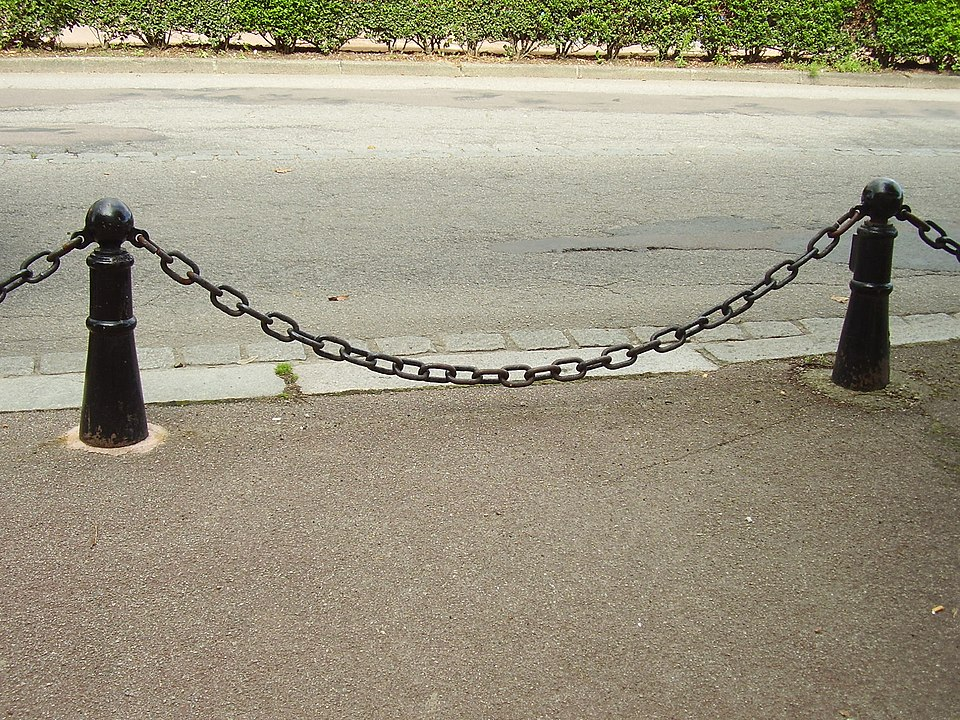
\includegraphics[scale=.2]{hanging_chain.jpg}

	\end{multicols}



  \item[\textbf{\underline{Physical Properties:}}] \hfill \vspace{0mm}
  
  Total Mass of Cable (not chain shown in image)
 	\[W = .048 (kg) \]
 	Total Length of Cable 
 	\[L = 147 (in) \]

  \item[\textbf{\underline{Boundary Conditions:}}] \hfill \vspace{0mm}
  
  \[y(x=0)=12, \hspace{2mm} y'(x=0)=0 \]
  \[y(x=-L/2)=y(x=L/2) \] 


  \item[\textbf{\underline{Measured Data:}}] \hfill \vspace{0mm}
 
   \begin{tabular}{|c|c|c|c|c|c|c|} \hline
   $x(in)$&0&12&24&36&48&60\\ \hline
   $y(in)$&12&13&16&23&33&48\\ \hline 
   \end{tabular}


\newpage
\item[\textbf{\underline{Activity:}}] \hfill \vspace{0mm}

Write a MATLAB program to approximate the displacement function of the catenary cable $y(x)$ using a curve fit model of your choice. Two methods will be used to generate the curve.

\begin{enumerate}	
	
	\item The numerical data should be hardcoded into the program, and the program should run without using user input. 

	\item Generate a curve fit function $y_1(x)$ to fit the data points with a model of your choice using the built-in MATLAB function {\it polyfit()} or other MATLAB curve fitting tool. You may need to install the MATLAB Curve fitting Toolbox. 

	\item Generate a second curve fit function $y_2(x)$ to fit the data points with a model of your choice using a custom MATLAB program. Suggested methods are Lagrange polynomials or polynomials as linear systems. Clearly state if the model for is different from the model used in part 2.

	\item Show the numerical data and both curve fits on the same figure. Use grid lines and label the axes.

	\item Bonus: Find an analytical solution to the problem using the physical properties and boundary conditions. Show all steps, and include a reference if applicable. Add the analytical curve to the results figure from part 3. Does the solution agree with the measured data?

\end{enumerate}

\newpage	



\item[\textbf{\underline{Submission:}}] \hfill \vspace{0mm}

	\begin{itemize}

		\item Submit the MATLAB program as a .m file. The program should run free from errors and produce the results described in the assignment including any figure. 

		\item Include answers to any discussion questions in a seperate document or the assignment submission textbox. 

	\end{itemize}		


		%Submit the most complete version of {\bf \BL<USERNAME>\BK\_activity\ANUM.pdf} \\and {\bf \BL<USERNAME>\BK\_activity6.m } to the Activity \ANUM \hspace{1mm} folder before the posted due date.

\end{description}
\end{document}
